%!TEX root = ../thesis.tex
%4-Snellen/Brogi analysis
% ability to detect singal??

\chapter{Spectral Companion Recovery}  % Main chapter title

\label{cha:model_comparison}

%----------------------------------------------------------------------------------------
%    SECTION 1
%----------------------------------------------------------------------------------------

Because the differential subtraction technique was unsuccessful, not being separable in time. A second method was attempted to try and extract something useful out of the spectra.

We develop this new method, preform some tests and then show the results obtained. There were numerous issues encountered and unsuccessful results.

Contrast our result to other works.  More phases, longer integration time, higher {SNR}.




\section{Main Section 1}
Model fitting two components.




\section{Binary synthetic spectral recovery}
\label{subsec:companion_recovery}
Since the differential method is ineffective for our dataset due to the {RV} separation between observations, we explored a second approach to detect the presence of the faint companion spectra. This second approach compares the observed spectra to combinations of synthetic spectral models using \textchisquared{} methods which have been extensively used in the literature~\citep[e.g.,][]{astudillo-defru_harps_2015, passegger_fundamental_2016, zechmeister_spectrum_2018, nemravova_xtauri_2016}. {\red{} The temperature of synthetic spectra fitted to  the companion will provide some indication of the companions spectral type, but will not produce a direct mass constraint that was the original aim of this work.}

\subsection{Synthetic {PHOENIX-ACES} models}
\label{subsec:spec_models}
We use the {PHOENIX-ACES}~\citep{husser_new_2013} synthetic spectra library as our reference for the spectral comparison. It uses the most recent version (16) of the PHOENIX code and is suitable for the spectra of cool stars. The full parameter grid space of the {PHOENIX-ACES} spectra is given in \tref{tab:phoenix} although we only explore models constrained by the targets explored here.

%!TEX root = ../thesis.tex

\begin{table}
    \centering 
    \caption{Full parameter space of the PHOENIX-ACES spectral grid.}
    \begin{tabular}{lr@{ -- }lc}    % Seperate columns with --
        \toprule
        & \multicolumn{2}{c}{Range}       & Step size\\
        %\midrule
        \midrule
        \ \(T_{\textrm{eff}}\) [K] &  2300 & 7000  & 100 \\
        &  7000 & 12000 & 200 \\ 
        \  logg     &  0.0 & +6.0   & 0.5 \\ 
        \ [Fe/H]   &  -4.0 & $-$2.0  & 1.0 \\    % Strange spacing of [ ] in table so added \ to all rows
        &  -2.0 & +1.0  & 0.5 \\  
        \  \(\alpha\)/Fe &  -0.2 & +1.2  & 0.2 \\
        \bottomrule
    \end{tabular}
    \label{tab:phoenix}
\end{table}

The spectral model libraries were accessed using the useful ``grid tools'' interface provided in the \emph{Starfish}\footnote{\url{https://github.com/iancze/Starfish}} Python package~\citep{czekala_constructing_2015}, which made it efficient to load in the spectra when needed.

We multiply the synthetic spectra by the wavelength to convert it into photon counts, ignoring multiplicative constants, as done in~\citet{figueira_radial_2016}\footnote{Synthetic models provide the spectral energy distribution (\(\rm erg\,s^{-1}\,cm^{2}\,cm^{-1}\)).}. The spectra were convolved with a Gaussian kernel to match the resolution of the observations (\(\rm R=50\,000\)). Due to the distributive property of convolution it is efficient to apply it once to each spectra first, before the spectral pairs are combined.

The {PHOENIX-ACES} models include dust in equilibrium with the gas phase while ignoring dust opacity and does not include any mixing/settling which is important for cooler {BD} atmospheres.
They set a minimum library \(\teff{}=2\,300\)\K{} to avoid the temperatures at which the modelling of clouds is necessary.
This unfortunately limits the use of this library for this technique to the largest mass companions in our sample.
For example a \(\teff{}=2\,300\)\K{} corresponds to a {BD} with \(\textrm{M}\sim84\)\Mjup{} at 5\Gyr{} from the~\citet{baraffe_evolutionary_2003} evolutionary models.

There are other models that extend below 2\,300\K{} such as the {BT-Settl} models\citep{allard_btsettl_2013,baraffe_new_2015}. These are discussed in \sref{subsubsec:BT-Settl}.


\subsection{\texorpdfstring{\textchisquared}\ \ method}
\label{subsec:chi2}
The well known \textchisquared{} technique measures the weighted sum of the squared deviation between the observation (\({O}_{i}\)) and the computed models (\(C_{i}\)), with the minimum \textchisquared{} value representing the best-fit parameters.
\[\chisquared = {\Sigma}_i {(O_{i} - C_{i})}^2 / {\sigma}_{i},\] where \({\sigma}_{i}\) is the error on each measurement. We estimate the \(\sigma\) of each spectrum using the \(\beta\sigma\) method~\citep{czesla_posteriori_2018}, using the MAD (median absolute deviation about the median) robust estimator. {\red{} This method estimates the spectral noise using numerical derivatives of the spectra. We followed the procedure outlined in~\citet{czesla_posteriori_2018}, analyzing the results from successive parameter combinations to settle on an order of approximation (derivative level) of 5, and a jump parameter (pixels skipped to avoid correlations) of 2.} We apply the same \(\sigma\) value to all points \({\sigma}_{i} = \sigma\).
The \(\beta\sigma\) method provided \(\sigma\) estimates for the target spectra which correspond inversely to signal-to-noise ratios between 100--500, {\red{} similar to the values given in \tref{tab:observations} calculated from the continuum of detector 2.}

The computed models are described in \sref{models} and result in a multidimensional grid of \textchisquared{} values for each combination of parameters, namely the spectral temperature, host {RV}, and companion {RV} for each detector, observation and target.

We obtain the global minimum of the multidimensional \textchisquared-space to represent the best fit to the observed spectra. We sum the multidimensional \textchisquared{} across multiple detectors and determine a global minimum \textchisquared{} for the whole observation \(\chisquared_{obs} = \Sigma^{N}_{n=1} \chisquared_n\), where \(N\) is the number of detectors used. We do not, however, combine the \textchisquared{} values across the separate observations as the {RV} parameters of the host and companion will vary between each observation. However, since the current observations are insufficiently separated, it may be possible to combine the separate observations; but in general this would not be the case, so was not performed.

The inverse survival function of the \textchisquared{} distribution is used to determine the confidence levels on the minimum \textchisquared{} parameters. The inverse survival function returns a \(\Delta\chisquared\) value from the minimum \textchisquared{} value for a given sigma level and degree of freedom\footnote{In \emph{Python} with the \emph{scipy} package this is a single line \texttt{scipy.stats.chi2{(dof)}.isf{(1-p)}}, where \(p = 0.68\) for 1-\(\sigma\), and dof is the degree of freedom.}.
For example, the \(\Delta \chisquared\) for a single degree of freedom required for the 1-, 2-, and 3-\(\sigma\) levels is 1, 4, and 9 respectively~\citep{bevington_data_2003}. This method assumes that the measured flux is observed with a {SNR} sufficiently high so that the noise on the spectrum is approximately Gaussian, and the \textchisquared{} method appropriate.

For a given observation, the \(\chisquared_{red}\) is computed by \(\chisquared_{red} = \chisquared / \nu\)where \(\nu = n - m\), the number of observed pixels, \(n\), minus the number of parameters of interest, \(m\)\footnote{\(m=2\) or 4 in the examples explored below}, and is performed after the summation over the detectors.



%%%%%%%%%%%%%%%%%%%%%%%%%%%%%%%%%%%%%%%%%%%%%%%%%%%%%%%%%%%%%%%%%%%%%%%%%%%%%%%
%%%%%%%%%%%%%%%%%%%%%%%%%%%%%%%%%%%%%%%%%%%%%%%%%%%%%%%%%%%%%%%%%%%%%%%%%%%%%%%

\subsection{Computed model spectra}
\label{models}
In this section we detail how we transform the synthetic {PHOENIX-ACES} spectra into the computed models (\(C_i\)) to fit to the observations. The spectra have already been converted to the correct unit and resolution.

These synthetic spectra are used individually for the single component model and combined together into a binary model. The results of these models are interpolated to the wavelength grid of the observed spectra and the \textchisquared{} calculated by comparing the model and observation at each point.


\subsubsection{Single component model}
\label{subsubsec:single-model}
The single model \(C^{1}_{i}\) comprises of a single synthetic spectrum, \(J\), (with model parameters \(\teff{}\), logg, \feh{}, [\(\alpha\)/\ce{Fe}]) and is Doppler shifted by a {RV} value \({rv}_1\).

\begin{equation}
\rm C^{1}_{i}(\lambda) = J(\lambda_0(1-\frac{{rv}_1}{c}))
\end{equation}

where \(\lambda\) is the shifted wavelength, \(\lambda_0\), the model rest wavelength and, \(c\), the speed of light in a vacuum. The model's flux is then continuum normalized to unity to match the observed spectra, and interpolated to the wavelength grid of the observation.

This single component model analysis is similar to the~\citet{passegger_fundamental_2016} \textchisquared{} fitting. We apply the same re-normalization (see \sref{subsec:renorm}) to account for slight differences in the continuum level and possible linear trends between the normalized observation and model. We do not, however, apply any dynamical masking to sensitive lines to make the the \textchisquared{} minima more distinct or linearly interpolate the stellar parameters between the grid models to obtain high precision stellar parameters. This is because we are not trying to derive precise stellar parameters but to detect the spectra of the companions. We instead include radial velocity components to the \textchisquared{} fitting, which is not included in~\citet{passegger_fundamental_2016}.


\subsubsection{Binary model}
\label{subsubsec:binary-model}
In the binary situation we consider the superposition of two synthetic spectral components, one each for the host and companion respectively. Both spectra are Doppler shifted by \({rv}_1\) which represents the {RV} motion of the host star, while the companion spectra is also Doppler shifted by a second {RV}, \({rv}_2\), representing the {RV} offset between the host and companion. This choice is arbitrary, but in this way the mean motion of the system relative to Earth is captured only in \({rv}_1\). The two spectra are scaled by their squared radius (see \sref{subsection-radius}) then added together, thus fixing the relative amplitude of the two components.
Given two spectral components \(J_{1}\)and \(J_{2}\)with radii \(R_1, R_2\) this equates to
\begin{align}
\rm C^{2}_{i}(\lambda) = &  J_{1}(\lambda_{0}(1 - \frac{rv_{1}}{c}))\times R_{1}^2 +\nonumber \\
& J_{2}(\lambda_{0}(1-\frac{rv_{1}}{c})(1-\frac{rv_{2}}{c}))\times R_{2}^2
\end{align}


The combined spectra is continuum normalized by dividing by an exponential fitted to the continuum of the combined spectrum, as we assume we are in the Rayleigh-Jeans regime. This assumption here is wavelength dependent and other appropriate continuum normalization techniques are also valid. In the case of a {BD} companion around an FGK star investigated here, the continuum is dominated by the contribution from the host star as it contributes the majority of the spectrum with flux ratios around 2\,110--2\,160\nm{} below \(\sim\)1\%.

We combine the models in this way to represent the correct absolute flux ratio of the components. The median flux ratio between the two components is calculated for the wavelength range used here as an indication of the flux ratio level.

The binary model should provide meaningful information about the companion parameters (e.g.\ \(\teff{}\)) and a estimate of the flux ratio of the system. These can be combined with the~\citet{baraffe_evolutionary_2003} models to constrain the mass of the companion. However, we need to be careful with this model as the inclusion of extra spectral components and associated parameters could also provide a better fit to observations which do not have a companion, by fitting components of the noise.\\

{\red{} The full list of grid parameters for the binary model are \(\teffsub{1}\),  \(\logg{}_1\), \feh{}\(_1\), [\(\alpha\)/\ce{Fe}]\(_1\), \({rv}_1\), \(\teffsub{2}\), \(\logg{}_2\), \feh{}\(_2\), [\(\alpha\)/\ce{Fe}]\(_2\), \({rv}_2\) where the subscripts 1 and 2 indicate the host and companion models respectively.}






\subsubsection{Effective radius}
\label{subsection-radius}

To combine the two synthetic spectra with the correct observed flux ratio we need to integrate the emitted flux over the effective surface area of each emitting body respectively. Ignoring the common multiplicative constants that will disappear with normalization, we scale the two synthetic spectra individually by the square of their respective radii, \(R_1\) and \(R_2\).

In this work we use the effective radius (PHXREFF keyword) of each component from the PHOENIX model headers. This is the radius used in modelling of the stellar atmospheres. We use this radii as it is directly tied to each model spectrum, and already available. The ratio of the radii from the two synthetic spectra in the binary models are provided in \tref{tab:example_params}.

We are aware that using these radii radii has its limitations, since as stated previously, there is a degeneracy in {BD} mass, age, and luminosity of the companion, and in particular a combination of radius-mass and radius-age relationships~\citep{sorahana_radii_2013}. Using the {PHOENIX-ACES} model effective radius does not allow for any independent age constraints to be incorporated, or allow for any variability in the radii to account for uncertainties.

The targets analysed here do not have transits, but if the radius ratio can be independently determined from the photometric transit method~\citep{deeg_photometric_1998} then this could be used to constrain the radius ratio used when combing the binary model spectra instead.


\subsection{Re-normalization}
\label{subsec:renorm}
Slight trends in the continuum level between the observed spectra and computed models were removed using the re-normalization following~\citep{passegger_fundamental_2016}:
\begin{equation}
F^{obs}_{re-norm} = F^{obs} \cdot \frac{\textrm{continuum fit}_{model}}{\textrm{continuum fit}_{observations}}.
\end{equation}
The polynomial continuum fits to the normalized observations and models are used to re-normalize the observed spectrum to the continuum of the models. For detectors 1--3 a polynomial of first degree was used, while for detector 4 a quadratic is needed to fit the edge of a strong Hydrogen line (Brackett-\(\gamma\)) at 2\,166\nm{}, which lies just off of detector 4. This broad line is only observed in the synthetic spectra and not in the reduced observations. It is assumed that this was normalized out during the reduction process.

For each model we further allow the continuum level to be varied by \(\pm 0.05\) as a free parameter taking the model with the smallest \textchisquared{} value.


\subsection{Reducing parameters}
\label{subsec:reduce-params}
The high dimensionality of the binary model makes it computationally challenging and difficult to analyse the \textchisquared{} space.
For reference, the multiplicative parameter space is squared when increasing from one spectral component in the single model to a binary model, and therefore becomes computationally expensive. In general the number of possible parameter combinations for \(c\) spectral components each with a grid of \(m\) models increases to \(c^m\). If the full set of {PHOENIX-ACES} library spectra (66456) is explored with a binary fit then this naively balloons to over 4.4 billion possible combinations. Half of these are not unique as the host and companion components are swapped. This is the worst case scenario and we implement a number of assumptions to vastly reduce the parameter-space enabling faster computation.

Our first assumption is to restrict ourselves to models with an Alpha element abundance ([\(\alpha\)/\ce{Fe}]) of zero. This is likely a very good approximation as all our targets have solar metallicity and are thus very likely to belong to the thin disk of the Galaxy, where [\(\alpha\)/\ce{Fe}] values are close to zero (i.e., solar) -- e.g.~\citet{adibekyan_chemical_2012}. Our second is to assume that we can significantly reduce the search space with literature values for the host star. We fix the metallicity of both components to the closest grid to the literature value (usually \feh{}=0.00). We also fix the \logg{} of the host star to its literature values given in \tref{tab:starparams}. The uncertainties on the literature measurements for \logg{} (\(\sim\)0.1) and metallicity (\(\sim\)0.05) are both smaller than the grid steps of 0.5 for these parameters.
For the \logg{} of the companion we use the~\citet{baraffe_evolutionary_2003,baraffe_new_2015} evolutionary model value for the given companions \(\textrm{M}_2\)/\(\textrm{M}_2\sin{i}\) and hosts age.

We use the estimated companion temperatures from the Baraffe evolutionary models given the companion \(\rm M_2\) or \(\textrm{M}_2\sin{i}\) and stellar age as a starting point for the companion spectra grid computation and extend the grid in each direction, within the model limits. For example we show the companion temperature grid spanning \(-600\) to \(+400\)\K{} in \fref{fig:Mdwarf_contours} and \(\pm400\)\K{} in Figs.~\ref{fig:HD211847_simulated_contours} and~\ref{fig:HD211847_result_contours}.

The large numbers stated above also do not include the {RV} grid for each component. The {RV} grid is user defined and the number of spectra /models to consider increases when the {RV} grid step size is decreased (finer {RV} resolution). We can reduce the {RV} grid space significantly by tailoring it to the target being examined. For each target, we use the estimated {RV} values from the observation time and orbital parameters, given in \tref{tab:observations} as a centre starting point for the \({rv}_1\) and \({rv}_2\) values and increment the {RV} within a few {\fwhm} around those values, or out to the targets \(\rm K_1\) and estimated \(\rm K_2\) values.

An iterative process could be implemented to refine the {RV} grids, starting at a larger grid with lower {RV} resolution then performing a higher resolution grid about the minimum \textchisquared{} {RV} values. This was only done manually but could have been automated. One could expect that a good starting {RV} grid step be governed by the spectral resolution, e.g.\ comparable to the {\fwhm} velocity.

For the companions targets with fully resolved orbits the known {RV} of  the host star, \({rv}_1\) could also have been fixed. We however left this free to see if the known value would be recovered by the fitting.





%%%%%%%%%%%%%%%%%%%%%%%%%%%%%%%%%%%%%%%%%%%%%%%%%%%%%%%%%%%%%%%%%%%%%
%%%%%%%%%%%%%%%%%%%%%%%%%%%%%%%%%%%%%%%%%%%%%%%%%%%%%%%%%%%%%%%%%%%%%


\section{Results}
\label{sec:results}

%!TEX root = ../thesis.tex

\begin{table*}
      \centering
      \begin{threeparttable}
          \caption{Input and recovered parameters on simulations and an observation when applying a single (\(\rm C^1\)) and binary (\(\rm C^2\)) models. The \logg{} and metallicity were fixed at \(\logg{}_1 = 4.50\), \(\logg{}_2=5.0\) and \feh{}=0.0 equally for both components. Gaussian noise was added to both simulations with a \snr{} of 150. Here \(m\) and \(n\) are the number of data points and parameters used in each model.}

          \begin{tabular}{c | *3c | *3c | *3c}
              \toprule
              & \multicolumn{3}{c|}{Simulation 1} & \multicolumn{3}{c|}{Simulation 2} & \multicolumn{3}{c}{Observed {HD 211847}} \\
              \midrule
          & Input & \multicolumn{2}{c|}{Recovered} & Input & \multicolumn{2}{c|}{Recovered} & Expected & \multicolumn{2}{c}{Recovered} \\
          & & \(C^1\) & \(C^2\) & & \(C^1\) & \(C^2\) & & \(C^1\)  & \(C^2\) \\
          \midrule
          \(\teffsub{1}\) & 5\,800 & 5\,800 & 5\,800 & 5\,700 & 5\,800 & 5\,700 & \(5\,715 \pm 24\) & 5\,900 & 5\,800\\
          \(\teffsub{2}\) & 4\,000 & -- & 3\,800 & 3\,200 & -- & 3\,100 & \(\sim\)3\,200 & -- & >3\,800\tnote{a}\\
          \({rv}_1\) & 0 & 0.1 & 0 & 6.6 & 6.6 & 6.6 & \(6.6 \pm 0.3\) & 7& 7.6 \\
          \({rv}_2\) &  10 & -- & 9.8 & 0.5 & -- &  -1& \(0.5 \pm 2\) & -- &-12.6\\
          \midrule
          \(R_1/R_2\)& 2.57 & -- & 2.71& 3.16 & - & 3.27 & 3.16 & -- & <2.71\tnote{a}\\
          \(\rm F_2/F_1\)& 0.084 & -- & 0.066 & 0.030 & -- & 0.026 & 0.030 & -- & >0.066\tnote{a}\\
          \(m\) & - & 3\,072 & 3\,072 & -- & 3\,072 & 3\,072 & -- & 2\,612 & 2\,612\\
          \(n\) & - & 2 & 4 & -- & 2 & 4 & -- & 2 & 4\\
          \textchisquared& -- & 4\,978 & 3\,792 & -- & 3\,746 & 3\,630  & -- & 37\,688 & 33\,860\\
          \(\chisquared_{red}\) & -- & 1.62 & 1.24 & -- & 1.22 & 1.18 & -- & 21.3 & 19.2\\
          {BIC} & -- & -20\,145 & -22\,315 & -- & -21\,477 & -21\,377& -- & 18\,281 & 14\,468\\
          \bottomrule
        \end{tabular}\label{tab:example_params}
        \begin{tablenotes}
            \item [a] {At the arbitrary upper limit for companion temperature grid (3\,800\K{}).}
        \end{tablenotes}
    \end{threeparttable}
\end{table*}

\missingfigure{includegraphics images/HD211847 example pcolors.pdf}

\begin{figure*}
    \centering
   % 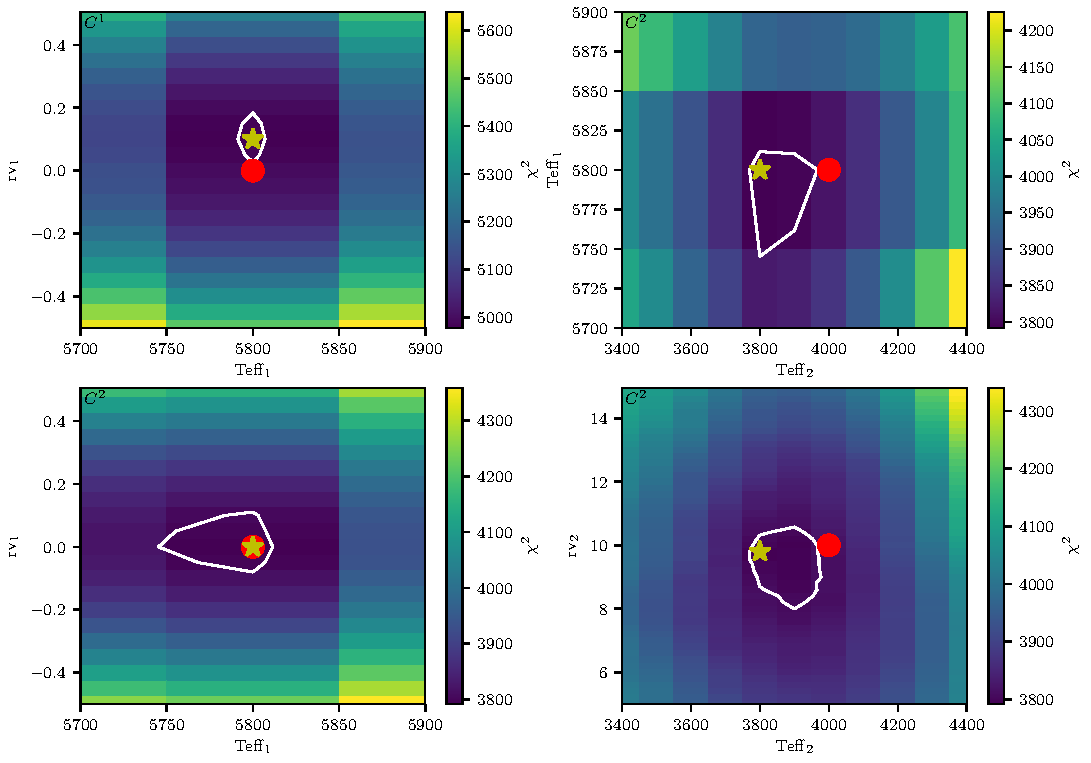
\includegraphics[width=0.8\hsize]{images/Mdwarf_pcolors.pdf}

    \caption{\textchisquared{} results for companion recovery of a simulated binary observation of a Sun-like star (\(\teffsub{1}=5\,800\)\K{}) with an M-dwarf companion (\(\teffsub{2}=4\,000\)\K{}). The top right plot shows the application of a single component model (\(C^1\)) while the other three are using a binary model (\(C^2\)). Both left hand panels show the distribution of host temperature and host {RV}.\@ The top right panel shows the distribution for host and companion temperature, and the bottom right the companion temperature and radial velocity.
        The red circle and yellow star indicate the location of the simulation input and recovered parameters respectively.
        The white line shows a 3-\(\sigma\) confidence level about the minimum \textchisquared{} solution grid point. Each box is centred on the parameter values and shows the grid resolution.}
    \label{fig:Mdwarf_contours}
\end{figure*}

\missingfigure{includegraphics {images/HD211847 example pcolors.pdf}}
\begin{figure*}
    \centering
   % 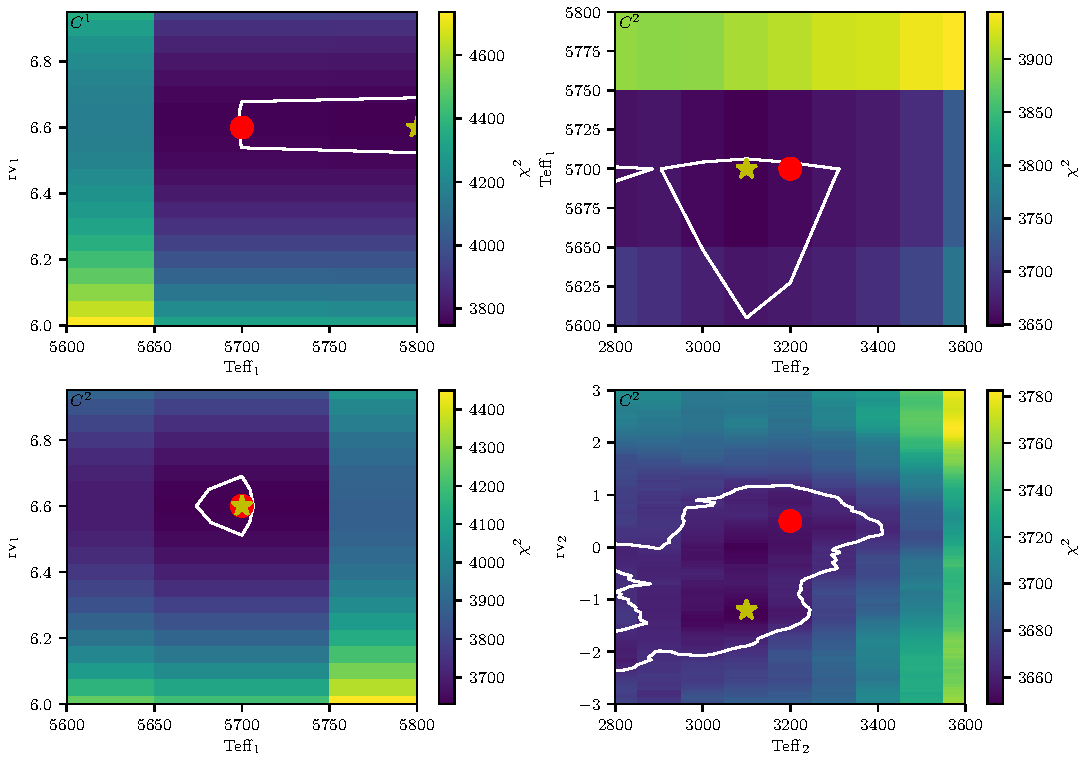
\includegraphics[width=0.8\hsize]{images/HD211847_example_pcolors.pdf}
    \caption{Similar to \fref{fig:Mdwarf_contours}, \textchisquared{} results for companion recovery of a simulated binary observation similar to {HD 211847}, (\(\teffsub{1} = 5\,800\)\K{}, \(\teffsub{2}=3\,200\)\K{}). The top right plot shows the application of a single component model (\(C^1\)) while the other three are using a binary model (\(C^2\)). Both left hand panels show the distribution of host temperature and host {RV}.\@ The top right panel shows the distribution for host and companion temperature, and the bottom right the companion temperature and radial velocity.
        The red circle and yellow star indicate the location of the simulation input and recovered parameters respectively.
        The white line shows a 3-\(\sigma\) confidence level about the minimum \textchisquared{} solution grid point. Each box is centred on the parameter values and shows the grid resolution.}
    \label{fig:HD211847_simulated_contours}
\end{figure*}
Here we show the results from applying the companion recovery model to simulated observations and to an observation.


\subsection{Simulated binaries}
\label{subsec:simulated_binaries}
To test the companion recovery method we create simulated binary observations using {PHOENIX-ACES} spectra. White noise was added with a standard deviation \(\rm \sigma = 1/{SNR}\), for a given signal-to-noise ({SNR}) level. We then applied the grid-matching recovery technique detailed above and compared the resulting parameters to the inputs.

The results of two example binary simulations are displayed in Figs.~\ref{fig:Mdwarf_contours} and~\ref{fig:HD211847_simulated_contours}, both simulated with a {SNR} of 150. The input and recovered parameters for the binary components are indicated by the red circles and yellow stars respectively, and are given in \tref{tab:example_params}.
The 3-\(\sigma\) contour is shown in white on the plots to indicate the shape of the confidence level only. The 1-\(\sigma\) contours are not shown here as they are much smaller than the temperature grid step and are not easy to visualize at this scale as they are often smaller than the marker shown at the minimum location. Each coloured rectangle is centred on the grid point, with its shape indicating the resolution of the grid space searched.

The first simulation shown in \fref{fig:Mdwarf_contours} is for a Sun-like star with a M-dwarf companion, with a \(\teffsub{2} =4\,000\)\K{}. The top-left panel shows the recovered host parameters when the single model is applied to the simulated binary. The top-right and both bottom panels are the parameters recovered when using the binary model. Both left-hand panels display the parameters for the host component to easily compare between models. With both models the host temperature \(\teffsub{1}\) is correctly recovered. The host {RV}, \({rv}_1\), is 0.1\kmps{} (two grid spaces) different from the simulated value for the single component model and is correctly recovered with the binary model.

The minimum \textchisquared{} location for the companion temperature is 200\K{} below the simulated value, and the {RV} of the companion recovered is 0.2\kmps{} below the input value. The input values for the companion are just outside of the 3-\(\sigma\) contours shown. The flux ratio for the input is 0.08 while the flux ratio recovered is 0.066.

The second simulation shown in \fref{fig:HD211847_simulated_contours} is performed with parameters to mimic the observation of our target with highest flux ratio, {HD 211847}. In this simulation the single component model recovers a host with the correct {RV} but a temperature 100\K{} higher than the input value. Again, adding the companion with the binary model recovers the correct host temperature. The companion temperature recovered is 100\K{} lower than the input temperature and the {RV} is different by 2\kmps{} which is around one third the {\fwhm}.

In this case with a companion {RV} offset, \({rv}_2\), near 0\kmps{} the host and companion lines are blended. The same spectral lines from both components are trying to match to the same features of the spectra, making it more difficult to recover the companion parameters. In the bottom right panel there appears to be multiple minima for different \({rv}_2\) and \(\teffsub{2}\) combinations, which we assume is partially due to the small \({rv}_2\).

In both simulations the reduced \(\chisquared_{red}\) for the binary model is closer to 1. This is not surprising as the binary model contains extra parameters. As mentioned above, we need to be careful, as the extra components from the binary may just happen to fit components of the noise when a binary is not present, or in our case has a low flux ratio.
{\red{} We analysis the significance between the two models using the ``Bayesian Information Criterion'' ({BIC})~\citep{schwarz_estimating_1978}; }
\begin{equation}
{BIC} = n\ln{(m)} - 2\ln{(\hat{L})}.
\end{equation}
{\red{} Here \(n\) and \(m\) are the number of parameters and data points respectively and \(\hat{L}\) is the maximum of the Gaussian likely-hood function }
\begin{equation}
\hat{L} = {\left(\frac{1}{\sigma \sqrt{2\pi}}\right)}^{m} \exp{\left(-\frac{\chisquared}{2}\right)},
\end{equation}
{\red{} written in terms of \textchisquared{} and a fixed \(\sigma\) for all data points. The maximum likely-hood of a Gaussian distribution is equivalent  to minimizing the \textchisquared. In both simulations \(\Delta {BIC} >10\) so the preference of the binary model, with the lower {BIC} value, over the single component model is considered \emph{significant}.}



\subsection{HD211847 observation}
\label{subsection:results-hd211847}
{HD 211847} is the best candidate for detection as it has a \(\rm 155~M_J\) low-mass star companion~\citet{moutou_eccentricity_2017}. The angular separation of the two bodies is 222 mas (or 11.3 au). Even though it is not a {BD} it has the highest estimated flux ratio in our sample, of 0.03 based on the~\citet{baraffe_new_2015} evolution models and the known companion mass (see. \tref{tab:estimatedparameters}). The angular separation of HD211847B is 222 mas with a projected distance of The result of applying \textchisquared{} fitting to the second observation of {HD 211847} is shown in \fref{fig:HD211847_result_contours}.

For this target the metallicity of both components was fixed to 0.0 and the \logg{} for the host was fixed at 4.5. The \logg{} for the companion is fixed to 5.0, based on the~\citet{baraffe_new_2015} evolutionary models for the given companion mass and system age. The orbital solution was used to refine the {RV} search space of both components. The span {RV} for the companion was extended until a value inside the {RV} bounds was found.

Again the top left panel of \fref{fig:HD211847_result_contours} shows the recovery with a single component model with the other three for the binary model. The single component model finds a temperature of 5\,900\K{} for the host with a \({rv}_1\) of 7\kmps{}. This is 200\K{} and 0.4\kmps{} different above the expected parameters. The binary model finds a host temperature of 5\,800\K{}, which is the second closest model to the literature value, >100\K{} different. The host {RV} value recovered with the binary model is 7.6\kmps{}, which is 1\kmps{} higher than expected.  For the single component model there is a barely noticeable secondary minima near this 7.6\kmps{} {RV} value recovered by the binary model. Again these {RV} differences are smaller than the {\fwhm} of the lines. The 3-\(\sigma\) contour is small, just visible on the right hand side of the star in the bottom left panel, and hidden behind the markers in the other panels.


For the companion in the binary model, on the right side of \fref{fig:HD211847_result_contours}, the minimum \textchisquared{} for the companion temperature is at the upper temperature limit of the grid shown. If we extend the grid of companion temperature towards higher temperatures the best fit location continues to increase in temperature, continually hitting the upper limit until it is close to the host temperature, >2\,000\K{} above the expected companion temperature. When the companion temperature becomes this high it also affects the recovered parameters for the host star to offset the features of the brighter companion.

The \(\chisquared_{red}\) values for the single and binary models are 21 and 19 respectively, far from 1, indicating that both models are a poor fit to the observations. {\red{} The $\Delta {BIC} = 3\,812 >10$ indicating that binary model is still preferred.} We plot the binary model for the best fit solution alongside the observed spectra in \fref{fig:visualinspection-hd2118471}. We see that there is a large spectral mismatch between the synthetic models and the observation. Extra wavelength masking was applied to many of the largest mismatched synthetic lines to remove their influence. The grey areas mark regions which have been masked out, either from the centres of deep telluric lines (the thin masks matching spectral gaps), or the more prominent mismatched lines in the synthetic spectrum excluded from the \textchisquared{} analysis. One clear example of a mismatched line is a synthetic line at 2\,132.5\nm{} that is clearly not observed in detector 2 (top right). Even with the majority of the mismatched lines removed the detection of the companion was still unsuccessful.

For detectors 1 and 2 it appears that the synthetic spectra contain many more deeper lines than observed. For detector 3 the red half of the detector was masked out as there appears to be an offset between the observed lines. With 3--4 lines that appear to be consistently offset from the observation it could be a wavelength calibration issue, although the telluric lines appear to be sufficiently corrected in this region, attesting for the quality of the wavelength calibration, and making it incompatible with the offset. For detector 4 the observed lines do not agree at all with the models. With many observed lines not in the model and only one line with some agreement in wavelength, detector 4 is masked out completely and not used in the \textchisquared{} fit. Individual inspection of the \textchisquared{} results for each detector also revealed that there was a large discrepancy between the 4th detector and the other three, with a different {RV} value for the host star and a \textchisquared{} values an order of magnitude higher. The edge of a deep Hydrogen line (Brackett-\(\gamma\)) off the edge of the detector 4 is also clearly seen in the continuum of the model >2\,162\nm{}.

We applied this same method to the remaining targets, with similar results. In brief, we conclude that the companion spectra cannot be correctly detected in our data using this method.
\missingfigure{images HD211847 result pcolors.pdf}
\begin{figure*}
    \centering
%    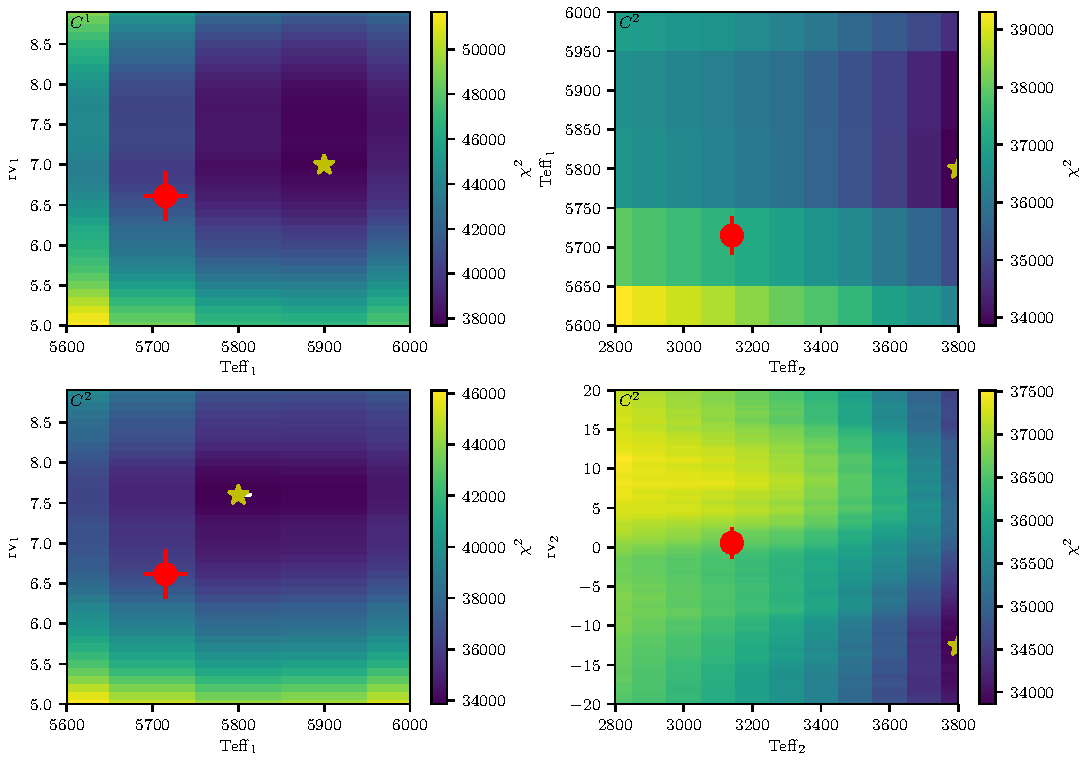
\includegraphics[width=0.8\hsize]{images/HD211847_result_pcolors.pdf}
    \caption{\textchisquared{} result grid for observation 2 of {HD 211847}, similar to Figs.~\ref{fig:Mdwarf_contours} and~\ref{fig:HD211847_simulated_contours}. The top right plot shows the application of a single component model (\(C^1\)) while the other three are using a binary model (\(C^2\)). Both left hand panels show the distribution of host temperature and host {RV}.\@ The top right panel shows the distribution for host and companion temperature, and the bottom right the companion temperature and radial velocity. The red circles indicate the literature values or calculated parameters for the target while the yellow star indicates the minimum \textchisquared{} solution. The error bar on the \(\teffsub{1}\) is from the literature while the error bars on \({rv}_1\) and \({rv}_2\) are calculated by propagating the orbital parameter uncertainties though the radial velocity equation. The white line shows a 3-\(\sigma\) confidence level about the minimum \textchisquared{} solution grid point, not always visible here due to the large \textchisquared{} values.}
    \label{fig:HD211847_result_contours}
\end{figure*}


\missingfigure{images/visualize result residuals.pdf}
\begin{figure*}
    \centering
  %  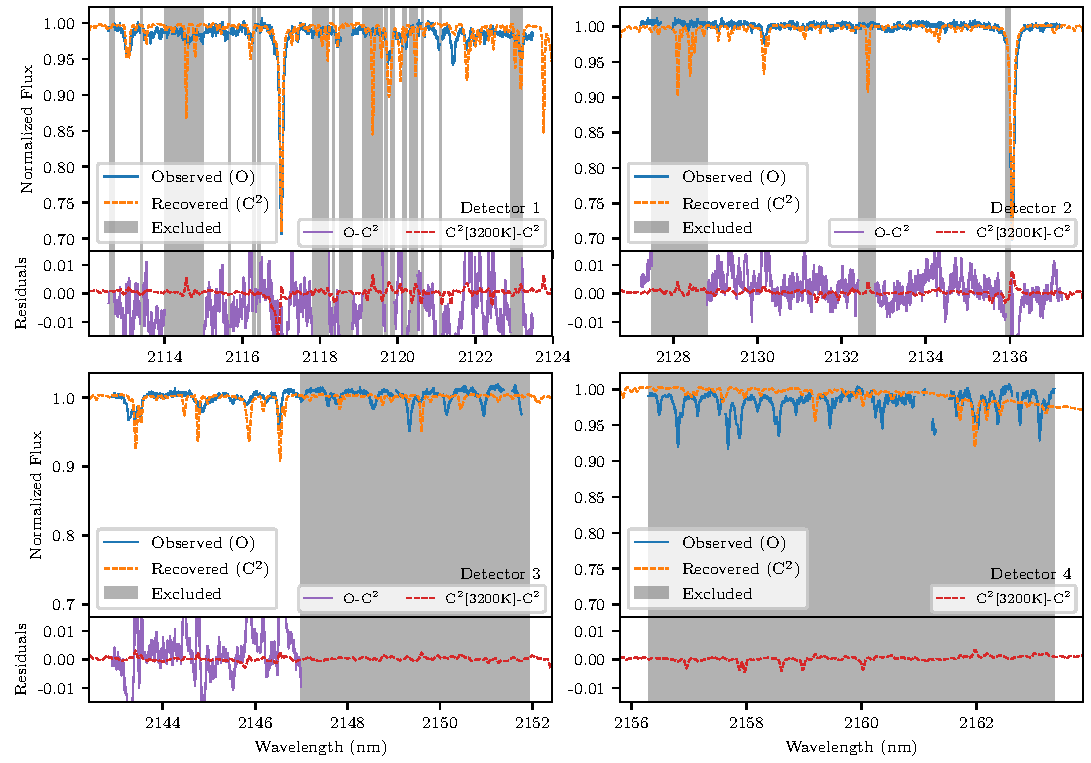
\includegraphics[width=0.8\hsize]{images/visualize_result_residuals.pdf}
    \caption{Comparison between the observed {HD 211847} spectrum (blue) and the best fit synthetic binary model (orange dashed) for each detector. The bottom section of each panel shows the residuals between the parts of the observation used in the \textchisquared{} fit and recovered binary model (\(\rm O-C^2\)) in purple. The red dashed line shows the difference between the recovered binary model and the binary model with the exact same parameters except for the estimated companion temperature of 3\,200\K{} (\(\rm C^2[3200\K{}]- C^2\)). The grey shading indicated the wavelength regions where masking has been applied. The thinner masked regions that match with cuts in the observed spectra are where the centres of deep (>5\%) telluric lines that have been masked out are.}
    \label{fig:visualinspection-hd2118471}
\end{figure*}


\subsection{Companion injection-recovery}
\label{subsection:injection-recovery}
To determine the detection limits for this method we employ an injection-recovery approach. We take the observed spectra and inject onto them a synthetic companion, at the absolute flux ratio to which it would have been added to a synthetic host with the same parameters. The injected companion {RV} is set to 100\kmps{} so that the companion lines are well separated from the lines of the host. This separation chosen is slightly larger than what we have with our observations, \(rv_2\) given in \tref{tab:observations}.

We restrict the search space by fixing the host parameters \(\teffsub{1}\) and \(\logg{}_1\) to those recovered fitting the non-injected spectra by a single component model. The wavelength masking is used to reduce the level of mismatch between synthetic and observed spectra.

We apply the recovery method developed above on the injected spectrum, leaving only the companion \(\teffsub{2}\) and \({rv}_2\) parameters free, to recover the injected companion. We repeated this for injected companions with temperatures below 5\,000\K{}.

We also perform the injection-recovery with synthetic host spectra, representing each target. The wavelength range of the synthetic spectra used for this is three sections interpolated to 1\,024 values in the wavelength span of detectors 1, 2, and 3. For each section, Gaussian noise is added at the level measured in the corresponding detector for the in the observation of the target being represented.

In \fref{fig:injection-recovery} we show the results of the injection-recovery on {HD 30501}. The blue dots represent the recovered companion temperature when injected into real observations, while the orange triangles represent injection into a synthetic host. Error bars of \(\pm100\)\K{} are included to indicate the grid size, and do not come from the recovery itself. The black dashed diagonal is the temperature 1:1 relation, where a correctly recovered companion should lie.

The grey shaded region indicates the \(\pm1\,000\)\K{} temperature range explored for the injection-recovery of the companion. This shows how the bounds of the grid are recovered at low temperatures.

For {HD 30501} the injection onto synthetic and observed spectra produce similar results. At temperatures above 3\,800\K{} in both the real and synthetic the injected companion is recovered within 100\K{}. For injected companion temperatures below 3\,800\K{} the temperature recovered is systematically higher than the injected value. This indicates that the companion is not correctly recovered and is affected by the added noise. We determine this temperature to be the upper temperature limit for the recovery. For the other stars we could not conclude on the upper limit due to spectral mismatch issues. In these cases we use the results from the synthetic injection to derive a temperature recovery cut-off for each target, each simulated with the closest host star spectrum.

In \fref{fig:injection_shape} we show the minimum \textchisquared{} for each companion temperature in the recovery grid. We do this for 7 different injected companion temperatures between 2\,500 and 4500\K{}. For the higher temperature companions, the \textchisquared{} is parabolic in shape, recovering the correct temperature, as expected. At lower temperatures there is a strong asymmetry in the \textchisquared{} with it flattening out on the lower temperature side.
The 1-, 2-, 3-\(\sigma\) values (with 2 degrees of freedom) of 2, 6 and 11 above the minimum \textchisquared{} are not shown in the bottom panel of \fref{fig:injection_shape} which is a close-up around the minimum \textchisquared{} as are indistinguishable in the top panel due to the \textchisquared{} y-scale. The black vertical line indicates the 2\,300\K{} temperature limit of the {PHOENIX-ACES} models.

\missingfigure{images/inject recovery hd30501.pdf}
\begin{figure}
    \centering
 %   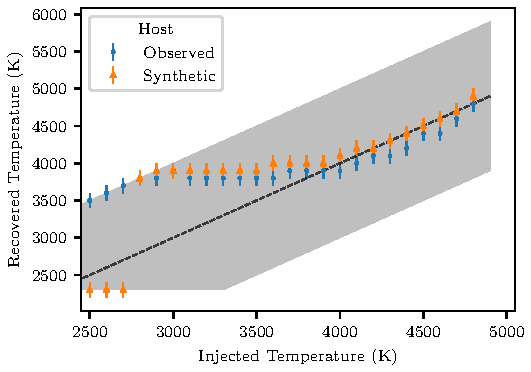
\includegraphics[width=0.95\hsize]{images/inject_recovery_hd30501.pdf}
    \caption{Result of simulated injection-recovery of synthetic companions on {HD 30501}. The blue dots and orange triangles indicate the recovered companion temperature for the observed and synthetic spectra respectively. The \(\pm100\)\K{} error bars are the grid step of the synthetic models. The black dashed diagonal shows the 1:1 temperature relation. The grey shaded region indicates the \(\pm1\,000\)\K{} temperature range explored. Gaussian noise added to the synthetic spectra was derived from the observed spectra.}
    \label{fig:injection-recovery}
\end{figure}


\missingfigure{images/chi2 shape investigation sigmas.pdf}
\begin{figure}
    \centering
%    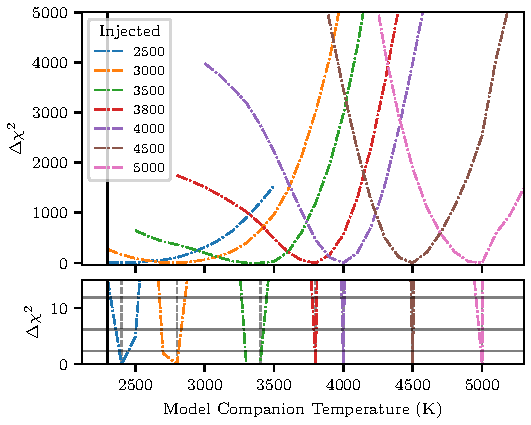
\includegraphics[width=0.95\hsize]{images/chi2_shape_investigation_sigmas.pdf}
    \caption{(top) Companion temperature verses \textchisquared{} for simulations with different injected companion temperatures. Other fixed parameters for these fully synthetic simulations was \(\teffsub{1}=5\,200\)\K{}, \(\textrm{logg}_1=4.5\), \(\textrm{logg}_2=5.0\), and both \feh{}=0.0. A fixed Gaussian noise corresponding to a {SNR} of 300 was used.
       (bottom) A close up view of \textchisquared{} < 15. The three horizontal grey lines indicate the 1, 2, 3 sigma with 2 degrees of freedom. The vertical dotted lines indicate the location of the minimum \textchisquared{} recovered for each companion. The black solid vertical in both panels shows the 2\,300\K{} cut-off of the {PHOENIX-ACES} models}
    \label{fig:injection_shape}
\end{figure}

%!TEX root = ../thesis.tex
\begin{table}
       \centering
  \begin{threeparttable}

       \caption{Upper mass limits of target companions assuming a companion \logg{}=5.0. Masses are derived from~\citet{baraffe_new_2015} evolutionary models using \(\teff{}\) and \logg{}. The flux ratio \(\rm F_2/F_1\) is  the absolute flux ratio between the cut-off temperature and the target host star.}

        \begin{tabular}{l c c c}
            \toprule
            Target & \txteff{} cut-off (K) & \(\rm F_2/F_1\) & Mass limit (\Mjup{})\\
            \midrule
            {HD 4747}     &  3\,900 & 0.084 & 598 \\
            {HD 162020} & 3\,900 & 0.147 & 598 \\
            {HD 167665} & 3\,800 & 0.054 & 560 \\
            {HD 168443} & 4\,000 & 0.094 & 618 \\
            {HD 202206} & 3\,900 & 0.075 & 598 \\
            {HD 211847} & 3\,900 & 0.079 & 598 \\
            {HD 30501}   & 3\,800\tnote{a} & 0.106 & 560 \\
            \bottomrule
        \end{tabular}
        \label{tab:mass_limits}
        \begin{tablenotes}[flushleft]
            \small
                \item [a] {From observed spectra }
        \end{tablenotes}
  \end{threeparttable}

\end{table}



Using the temperature cut-off values, we derive an upper mass limit for the companions around our stars using the~\citet{baraffe_new_2015} evolutionary models, finding the closest point matching the spectral temperature cut-off and \(\logg{}=5.0\). These values are given in \tref{tab:mass_limits} and are between 560 and 618~\Mjup{}. The flux ratio between the cut-off and the host star are also provided for, being between 5 and 15\% in this wavelength span.




% DISCUSSION









\subsection{Junk from paper about BT-settl}


\textbf{Alot of this section needs to be cut out, lots of repeats and it is not well structured. Basically it will say there is this other model that is better for BDs as it differs ``like this'' but Fig.~\textbf{ref {fig:hd211847-models}} show that it will also have strong mismatch to make it difficult to recover.}

\label{bt-setll}
The {BT-Settl} (allard et al 2009, 2010 2011 2012 baraffe2015) models, a different flavour of Phoenix models, are more suitable for {BD} atmospheres as they include the formation of dust/cloud and hydro-dynamical modelling atmospheric mixing/settling for atmospheres with \(\teff{}\) below \(\sim2600\K{}\). These are valid across the regime from stars to BDs as cool as 400\K{}. The {PHOENIX-ACES} models completely avoid the modeling of clouds and settling by the lower temperature restriction of 2\,300\K{}.

The {PHOENIX-ACES} models dust in equilibrium with the gas phase but ignores the dust opacity and does not include any settling. It does however include a new Astrophysical Chemical Equilibrium Solver (ACES,
Barman 2012); adds parametrisations for the mass and mixing-length; and uses the~\citet{asplund_chemical_2009} solar abundances. All these modifications together make it difficult to quantify the spectral changes from each individual change.

The two of the recent ``flavors'' are the {BT-Settl}~\citep{allard_model_2010, baraffe_new_2015} and the {PHOENIX-ACES}~\citep{husser_new_2013} which use versions 15.5 and 16 of the PHOENIX code respectively.

Even though the {BT-Settl} models are more suited for the entire range of {BD} temperatures, we restrict ourselves to the {PHOENIX-ACES} synthetic spectra for a number of reasons. The ease of use and availability from the spectral library webpage\footnote{\url{http://phoenix.astro.physik.uni-goettingen.de/?page_id=15}}. The ease of use using the Starfish tools, a wide parameter range and fairly consistent parameter grid span, and the effective radius of the modelled star provided in the fits header.

These were not used in this instance for a couple of reasons, the ineffectiveness to produce a reliable detection on the observations using PHOENIX ACES spectra for our largest companions, which fall well within the PHOENIX ACES temperature limit.

The {PHOENIX-ACES} models also provide dimensions of effective radius of the star, in the header. This is required for the method presented here as we need to scale the spectra by their respective surface area when combining together.
This {PHOENIX-ACES} lower temperature limit restricts its use to only the higher mass {BD} companions in our sample (\(~>0.08 M_{\odot}\) at 5\Gyr{} from the~\citet{baraffe_evolutionary_2003} models).


The most recent {BT-Settl} spectral library designated CIFIST2011\_2015\footnote{\url{https://phoenix.ens-lyon.fr/Grids/{BT-Settl}/CIFIST2011_2015/}}~\citep{baraffe_new_2015} is only available for 1\,200--7\,000\K{}\logg{}=2.5 to 5.5 and a fixed metallicity and alpha of 0 and includes newer Caffau et al. (2011) solar abundances.

The newer {PHOENIX-ACES} models are limited to \(\teff{}> 2\,300\)\K{} which only cover the larger BDs. To evaluate the lower mass BDs we use the \textbf{other model}, more suitable for cooler BDs and low mass star as they incorporate modeling of dust, clouds etc\ldots


The spectral model libraries were accessed using the useful ``grid tools'' provided in the Starfish\footnote{\url{https://github.com/iancze/Starfish}} Python package\citep{czekala_constructing_2015}.


Both sets of synthetic models do not handle the affects of radiation from a neighbouring star, which may have an affect on the binary orbits here.



{PHOENIX-ACES} models dust in equilibrium with gas phase but ignores the dust opacity and does not include any mixing/settling in cooler atmospheres. This is avoided by having a minimum library \(\teff{}=2\,300\)\K{}. This unfortunately limits the use of this library for this technique to the larger mass companions in our sample. For example a \(\teff{}=2300\)\K{} corresponds to a {BD} with M\(\sim0.08\)\Modot at 5\Gyr{} from the~\citet{baraffe_evolutionary_2003} evolutionary models.


Even though the {BT-Settl} models are more suited for the entire range of {BD} temperatures down to 400\K{}, through hydrodynamically modeling the mixing and settling of dust/clouds, we restrict ourselves to the {PHOENIX-ACES} synthetic spectra in this work for a number of reasons. The ease of use and availability from the spectral library webpage\footnote{\url{http://phoenix.astro.physik.uni-goettingen.de/?page_id=15}}. The effective radius of the modelled star are provided in the fits header and required for the calculation of the flux ratio.



The most recent {BT-Settl} spectral library designated CIFIST2011\_2015\footnote{\url{https://phoenix.ens-lyon.fr/Grids/{BT-Settl}/CIFIST2011_2015/}}~\citep{baraffe_new_2015} is only available for 1\,200-7\,000\K{}\logg{}=2.5 to 5.5 and a fixed metallicity and alpha of 0 and includes newer Caffau et al. (2011) solar abundances.

The {BT-Settl} grids were harder to obtain and use.

As we do not recover suitable results for HD211847 which is supposed to have a temperature around 3\,400\K{} we suspect that it is not possible for lower temperature either so don't try to extend to the {BT-Settl} models.


\textbf{
    PHOENIX ACES defines grid as Teff,\logg{} and Mass which can then be used to determine Radii. See~\citep{husser_new_2013} section 2.3.1 Mass.}

Both {BT-Settl} and aces are spherical
\ldots{}




\subsection{Incremental changes}
\textbf{incremental changes in models are small}

We took the synthetic models and investigated how the synthetic binary changed as the model parameters were incremented.  For the temperature of the companion to be incremented by 100\K{} this resulted in change to the spectrum with a std of XXX. This is around a {SNR} of around 500.
The change in the models with incremental changes in temperature is small, Changes in log and feh are larger but we fixed these for the application above.





\subsection{Note about a target - discussion of results}
Another example is \object{HD 162020}, which has the lowest orbital period (8.4 days) of our targets. It should have been possible to obtain an optimal pair of observations in one semester, but the second observation was taken immediately following the first. This means that the \(\rm \delta {RV} = 0.363\kmps{}\)between the two observations, is comparable to the \(\Delta {RV}\)that occurs during each individual observation. With tighter scheduling restrictions this target could have been observed with the optimal {RV} separation at the extrema of \(\Delta {RV}=2 K_{2}\)). Whether the flux ratio of \(7e^{-6}\) for this target and the interaction of different spectral lines would have made it possible to recover companion mass is a separate issue.



\subsubsection{Wavelength range}
The wavelength choice for the spectra analysed here, observed with the intention to apply the spectral differential technique, was selected due to the location of the \emph{K}-band telluric absorption window. This wavelength range, with a narrow wavelength range \(\sim50\)\nm{} set by the {CRIRES} instrument. This wavelength range is likely not the best choice for the proposed study. \todo{finish this line} may contribute to the poor results from the companion recovery technique.

For instance~\citet{passegger_fundamental_2016} used four different spectral regions for the precise parameter determination of M-dwarfs. Specific lines from the different wavelength regions are affected differently by the model parameters: \(\teff{}\), \logg{}, and \feh{}; and are used to break degeneracies in the {PHOENIX-ACES} parameter space.

Changing the wavelength coverage to regions with lines sensitive to stellar parameters for both stars and BDs, as well as using a larger wavelength range that will be achieved by {CRIRES+}, may help to improve the recovery results of the companion recovery technique presented here. We note that if the wavelength range is increased by taking separate observations at different wavelengths, not covered by a single exposure, then changes in the {RV} of both components between the different wavelength observations may need to be accounted for.







Try some Cross-correlations on simulations.

\todo{Try cross correlation at a different wavelength 2.3 micron?}
\todo{Try cross correlation with much larger wavelength range. 50, 100, 600, 1\,000 nanometres?}

\todo{Try my simulations with much larger wavelength range. 50, 100, 600 nanometres?}
